\documentclass[BCOR0mm,fontsize=12pt,paper=a4,final,numbers=noenddot]{scrartcl}
%\usepackage[T1]{fontenc} % Für PDFLaTeX
\usepackage[utf8]{inputenc} 
\usepackage[hyphens]{url}
\usepackage[ngerman]{babel}
\usepackage{amsmath}
\usepackage{amssymb}
\usepackage[style=german]{csquotes}
\usepackage{setspace}
\usepackage{tocloft}
\usepackage[medium]{titlesec}
\usepackage{color}
\usepackage[colorlinks=true,linkcolor=black,anchorcolor=black,citecolor=black,filecolor=black,menucolor=black,urlcolor=black]{hyperref}
\usepackage[inner=2.2cm,outer=2.2cm,top=2cm,bottom=2cm,includefoot,footskip=14mm]{geometry}
\usepackage{scrpage2}
\usepackage[final]{microtype}
\usepackage{soul}
\usepackage{blindtext}
\usepackage{paralist}
\usepackage{upgreek}
\usepackage{lscape}
\usepackage{enumitem} 
\usepackage{longtable}
\usepackage{tabu}
\usepackage[]{listings}
\usepackage{graphicx}
\usepackage{tikz-er2}
\usepackage{verbatim}
\usepackage{ulem}
\usepackage{pythonhighlight}


% Einstellungen für Listings
\definecolor{grey}{rgb}{0.4, 0.45, 0.41}
\lstset{language=Java,
                basicstyle=\ttfamily\footnotesize,
                keywordstyle=\color{blue}\ttfamily,
                stringstyle=\color{red}\ttfamily,
                commentstyle=\color{grey}\ttfamily,
                morecomment=[l][\color{grey}]{\#},
                showstringspaces=false}

\pagestyle{plain}

% Auslassungszeichen

\renewcommand{\dots}{[\ldots]}

\begin{document}
\makeatletter         

% Kapitelüberschriften
\renewcommand*{\thesubsection}{\@arabic\c@subsection.}
\renewcommand*{\thesubsubsection}{\@alph\c@subsubsection)}
\titleformat{\section}[hang]{\sffamily\bfseries\LARGE\centering}{\thesection}{5pt}{}
\titleformat{\subsection}[hang]{\sffamily\bfseries\Large}{\thesubsection}{5pt}{}
%\titleformat{\subsubsection}[hang]{\sffamily\bfseries\Large}{\thesubsubsection}{5pt}{}
%\renewcommand*{\raggedsection}{\centering}


\makeatother


\setlength{\baselineskip}{11pt}

\noindent{}\begin{footnotesize}Freie Universität Berlin\\
Institut für Informatik\\
Datenbanksysteme\\
Sommersemester 2017\\
Bearbeiter: Felix Binder, Nicolas Höcker, Armin Weber\\
\end{footnotesize}

\setlength{\baselineskip}{12pt}

\bigskip

\section*{Projektdokumentation}

\onehalfspacing

\subsection{Projektziel}

Ziel des Projekts ist es, eine "`Projekt"=Web"=Anwendung"' zu erstellen, mit deren Hilfe der Datensatz "`american"=election"=tweets"' analysiert werden kann. Analysieren heißt hier, dass die Anwendung in der Lage sein soll, das Beziehungsgeflecht zwischen den in den Tweets verwendeten Hashtags grafisch darzustellen und mittels benutzerdefinierter Anfragen weitere Informationen aus den Daten zu gewinnen. So soll es unter anderem möglich sein, die am meisten verwendeten Hashtags zu identifizieren, Aussagen über deren paarweise gemeinsames Auftreten zu treffen und die Wichtigkeit einzelner Tweets zu bewerten. Auch Auswertungen dessen, wie sich die einzelnen Punkte über die Zeit hinweg verändert haben, sollen möglich sein.

% (Anmerkung für uns: Das Projekt hat also zwei Seiten: 1. Das ganze technisch umsetzen. 2. Nebenbei ein Maß für zunächst rein semantische Sachverhalte wie "`Wichtigkeit"' finden, so dass sich Daten aus dem Datensatz gewichten lassen.)

\subsection{Team}

\paragraph*{Felix Binder:} Studiert Philosophie und Informatik (60 LP) gegen Ende seines Bachelorstudiums.

\paragraph*{Nicolas Höcker:} Studiert Informatik im 4. Bachelorsemester.

\paragraph*{Armin Weber:} Studiert Informatik im vierten Semester.


\subsection{Explorative Datenanalyse}

Der Datensatz besteht aus 6126 Tweets, die zwischen dem 5.~Januar 2016 und dem 28.~September 2016 über die Twitter"=Konten \textit{realDonaldTrump} und \textit{HillaryClinton} abgesetzt, d.\,\,h. von diesen selbst verfasst oder retweetet wurden. Das jeweilige Twitter"=Konto findet sich dabei in der ersten Spalte des Datensatzes ("`handle"'); die Information, ob es sich um einen Retweet handelt, in der dritten Spalte ("`is\_retweet"'), in der vierten bei Retweets der ursprüngliche Autor ("`original\_author"'). Der Text selbst -- und mit ihm alle Hashtags -- befindet sich in der zweiten Spalte.

Darüber hinaus enthält der Datensatz Informationen darüber, ob der Text ein Zitat ist und also auf eine andere Quelle verweist (siebte Spalte, "`is\_quote\_status"', mit der Quelle in der neunten Spalte, "`source\_url"') sowie dabei evtl. abgekürzt wurde (zehnte Spalte, "`truncated"'), ob der jeweilige Tweet eine Antwort auf einen anderen Tweet darstellt (sechste Spalte, "`in\_reply\_to\_screen\_name"'), wie oft er retweetet wurde und wie oft favorisiert (Spalten 7 und 8).

Dem ersten Augenschein nach sind für uns von Bedeutung:

\begin{enumerate}[label=\alph*),nosep]
 \item die Spalte Text, um daraus die Hashtags zu extrahieren;
 \item die Spalte mit dem Datum und der Uhrzeit, um das unterschiedlich starke Vorkommen von Hashtags zu verschiedenen Zeitpunkten nachvollziehen zu können;
 \item die Spalten zu Retweets und Favorisierungen, weil sie Indikatoren für die Wichtigkeit von Tweets sind.
\end{enumerate}

Die weiteren Spalten scheinen auf den ersten Blick für unsere Zwecke vernachlässigbar zu sein.


\clearpage

\subsection{ER"=Modellierung}

Das ER"=Modell für das Projekt sieht wie folgt aus:

\bigskip

\usetikzlibrary{positioning}
\usetikzlibrary{shadows}

\begin{footnotesize}

\begin{tikzpicture}[node distance=4em]
 \node[entity] (tweet) {Tweet};
    \node[attribute] (handle) [above=9em of tweet] {handle} edge (tweet);
    \node[attribute] (id) [below left=2cm of tweet] {\key{ID}} edge (tweet);
    \node[attribute] (text) [above= 6em of id] {text} edge (tweet);
    \node[attribute] (time) [above=2em of id] {time} edge (tweet);
    \node[attribute] (is_q) [above= 10em of id,align=center] {is\_quote\_\\status} edge (tweet);
    \node[attribute] (favorite_count) [above=16em of id] {favorite\_count} edge (tweet.120);
    \node[derived attribute] (imp) [right=of handle] {Wichtigkeit} edge (tweet);
    \node[attribute] (retweet_count) [below=2em of id] {retweet\_count} edge (tweet);
    \node[attribute] (is_r) [below=8em of tweet] {is\_retweet} edge (tweet);
 
%  \node[relationship] (schreibt) [above=2cm of tweet] {schreibt} edge [total] node[auto,swap]{N} (tweet);
%  
%  \node[entity] (autor) [above=2cm of schreibt] {Autor} edge node[auto,swap]{1} (schreibt);
%     \node[attribute] (hanlde) [left=of autor] {\key{handle}} edge (autor);
%     
%  \node[relationship] (retweetet) [right=0.4cm of schreibt] {retweetet} edge node[auto,swap]{1} (autor);
%     \node[attribute] (orig) [above right=of retweetet] {original\_author} edge (retweetet);
%     \draw[link]  (tweet)  -/ node[left,swap]{N} (retweetet);
%     
 \node[relationship] (enth) [right=2cm of tweet] {enthält} edge node[auto,swap]{N} (tweet);
    \node[attribute] (oft) [above right=of enth] {wie\_oft} edge (enth);
 \node[entity] (hash) [right=2cm of enth] {Hashtag} edge [total] node[auto,swap]{M} (enth);
    \node[attribute] (name) [above=of hash] {\key{Name}} edge (hash);
    \node[attribute] (anz) [above right=0.7cm of hash, align=center] {Anzahl\_\\global} edge (hash);
 
 \node[relationship] (bilden) [below=1.4cm of hash] {bilden} edge node[auto,swap]{2} (hash);
 
 \node[relationship] (ent) [below right=3cm of tweet] {enthält} edge node[auto,swap]{N} (tweet);
    \node[attribute] (w_oft) [below=of ent] {wie\_oft} edge (ent);
    
 \node[entity] (hash_p) [below=5cm of hash,align=center] {Hashtag-\\Paare} edge [total] node[auto,swap]{M} (ent);
    \node[attribute] (anzahl) [below= of hash_p] {Anzahl\_global} edge (hash_p);
    \node[attribute] (hp_id) [below right=1cm of hash_p] {\key{ID}} edge (hash_p);
    \node[attribute] (name2) [right=0.4cm of hash_p] {name2} edge (hash_p);
    \node[attribute] (name1) [above right=1cm of hash_p] {name1} edge (hash_p);
    
 \draw[link] [total] (bilden)  -/ node[right,swap]{M} (hash_p);
    
\end{tikzpicture}

\end{footnotesize}

\noindent{}Dieses Modell enthält augenblicklich noch mehr Informationen, als für die Beantwortung der in Abschnitt 1 genannten Fragen nötig wäre. So wäre es eigentlich unnötig abzuspeichern, ob ein Tweet ein Retweet oder ein Zitat ist. Allerdings wollen wir die Option offenhalten, in der fertigen Anwendung zu untersuchen, ob es signifikante Unterschiede hinsichtlich der Wichtigkeit der Tweets der verschiedenen Arten gibt. Da wir solche Unterschiede nicht ausschließen können, scheint uns das Weglassen solcher Informationen zu diesem frühen Zeitpunkt nicht angeraten.

Davon abgesehen war unser Anliegen, immer die naheliegenden Entscheidungen zu treffen: etwa Hashtag"=Paare aus Hashtags zusammenzusetzen und in den Relationen alle Informationen zu speichern, die später abrufbar sein sollen, etwa wie oft Hashtags in einzelnen Tweets vorkommen. Dort, wo es sinnvoll erschien, haben wir als Schlüssel außerdem eigenständige IDs ergänzt, um keine zu komplexen Schlüssel verwenden zu müssen (wie es bei den Tweets sonst etwa der Fall wäre).

Außerdem haben wir uns nach einigem Hin und Her dazu entschlossen, den Autor eines Tweets als Attribut handle in das Modell zu integrieren statt als eigene Entität. Hätten wir ihn als eigene Entität modelliert, die zu Tweets in den Relationen "`schreibt"' und "`retweetet"' steht, so hätten wir eine Tabelle mit nur einem einzigen Attribut (eben "`handle"'), wohingegen alle Attribute der Relationen zu "`Tweet"' gezogen hätten werden können, da es sich um 1:N"=Relationen gehandelt hätte. Damit hätte man für Abfragen nach dem Autor eines Tweets eigens mehrere Tabellen mittels JOIN verbinden müssen, was gerade bei Abfragen von den Hashtags her reichlich komplex geworden wäre, ohne dass das Ausgliedern des Autors als Entität irgendeinen Vorteil zu versprechen schien.


\subsection{Relationales Modell}

\noindent\textsc{Tweet}(\uline{ID}, handle, text, time, is\_retweet, is\_quote\_status, retweet\_count, favorite\_count)

\noindent\textsc{Hashtag}(\uline{Name}, Anzahl\_global)

\noindent\textsc{T\_enth\_H}(\uline{\dashuline{Tweet\_ID}, \dashuline{H\_Name}}, wie\_oft)

\noindent\textsc{Hashtag\_Paare}(\uline{ID}, Anzahl\_global, \dashuline{name1}, \dashuline{name2})

\noindent\textsc{Hashtags\_bilden\_HP}(\uline{\dashuline{Hash\_Name}, \dashuline{HP\_ID}})

\noindent\textsc{T\_enth\_HP}(\uline{\dashuline{Tweet\_ID}, \dashuline{Hashpaar\_ID}}, wie\_oft)

\medskip\noindent{}Grundsätzlich haben wir uns bei der Erarbeitung des relationalen Modells an die systematische Umwandlung aus der Vorlesung bzw. den Tutorien gehalten. Neben der korrekten formalen Übertragung und der daraus resultierenden funktionalen Bedeutung der Tabellen waren uns eine einleuchtende Benennung und eine gute Strukturierung wichtig, die Dritten das Verständnis erleichtert. Die Benennung der Tabellen haben wir so gestaltet, dass man aus den Namen möglichst sofort die inhaltliche Bedeutung ablesen kann. Dies war besonders für die beiden "`enthält"'"=Relationen aus dem ER-Modell wichtig. Auch die zusammengesetzten Primärschlüssel der Relationstabellen haben wir klar benannt. Bei allen Relationstabellen haben wir uns für einen zusammengesetzten Primärschlüssel aus den verbundenen Entitätstabellen und damit auch überhaupt für die Beibehaltung derselben entschieden. Die Möglichkeit, die Relationen direkt in eine Entität auszulagern, erschien uns zu unstrukturiert und schlechter erfassbar für Dritte, die unsere Datenbank schnell verstehen möchten. 

\clearpage

\subsection{Datenbank}
Wir haben eine Datenbank \textit{Election} erstellt.

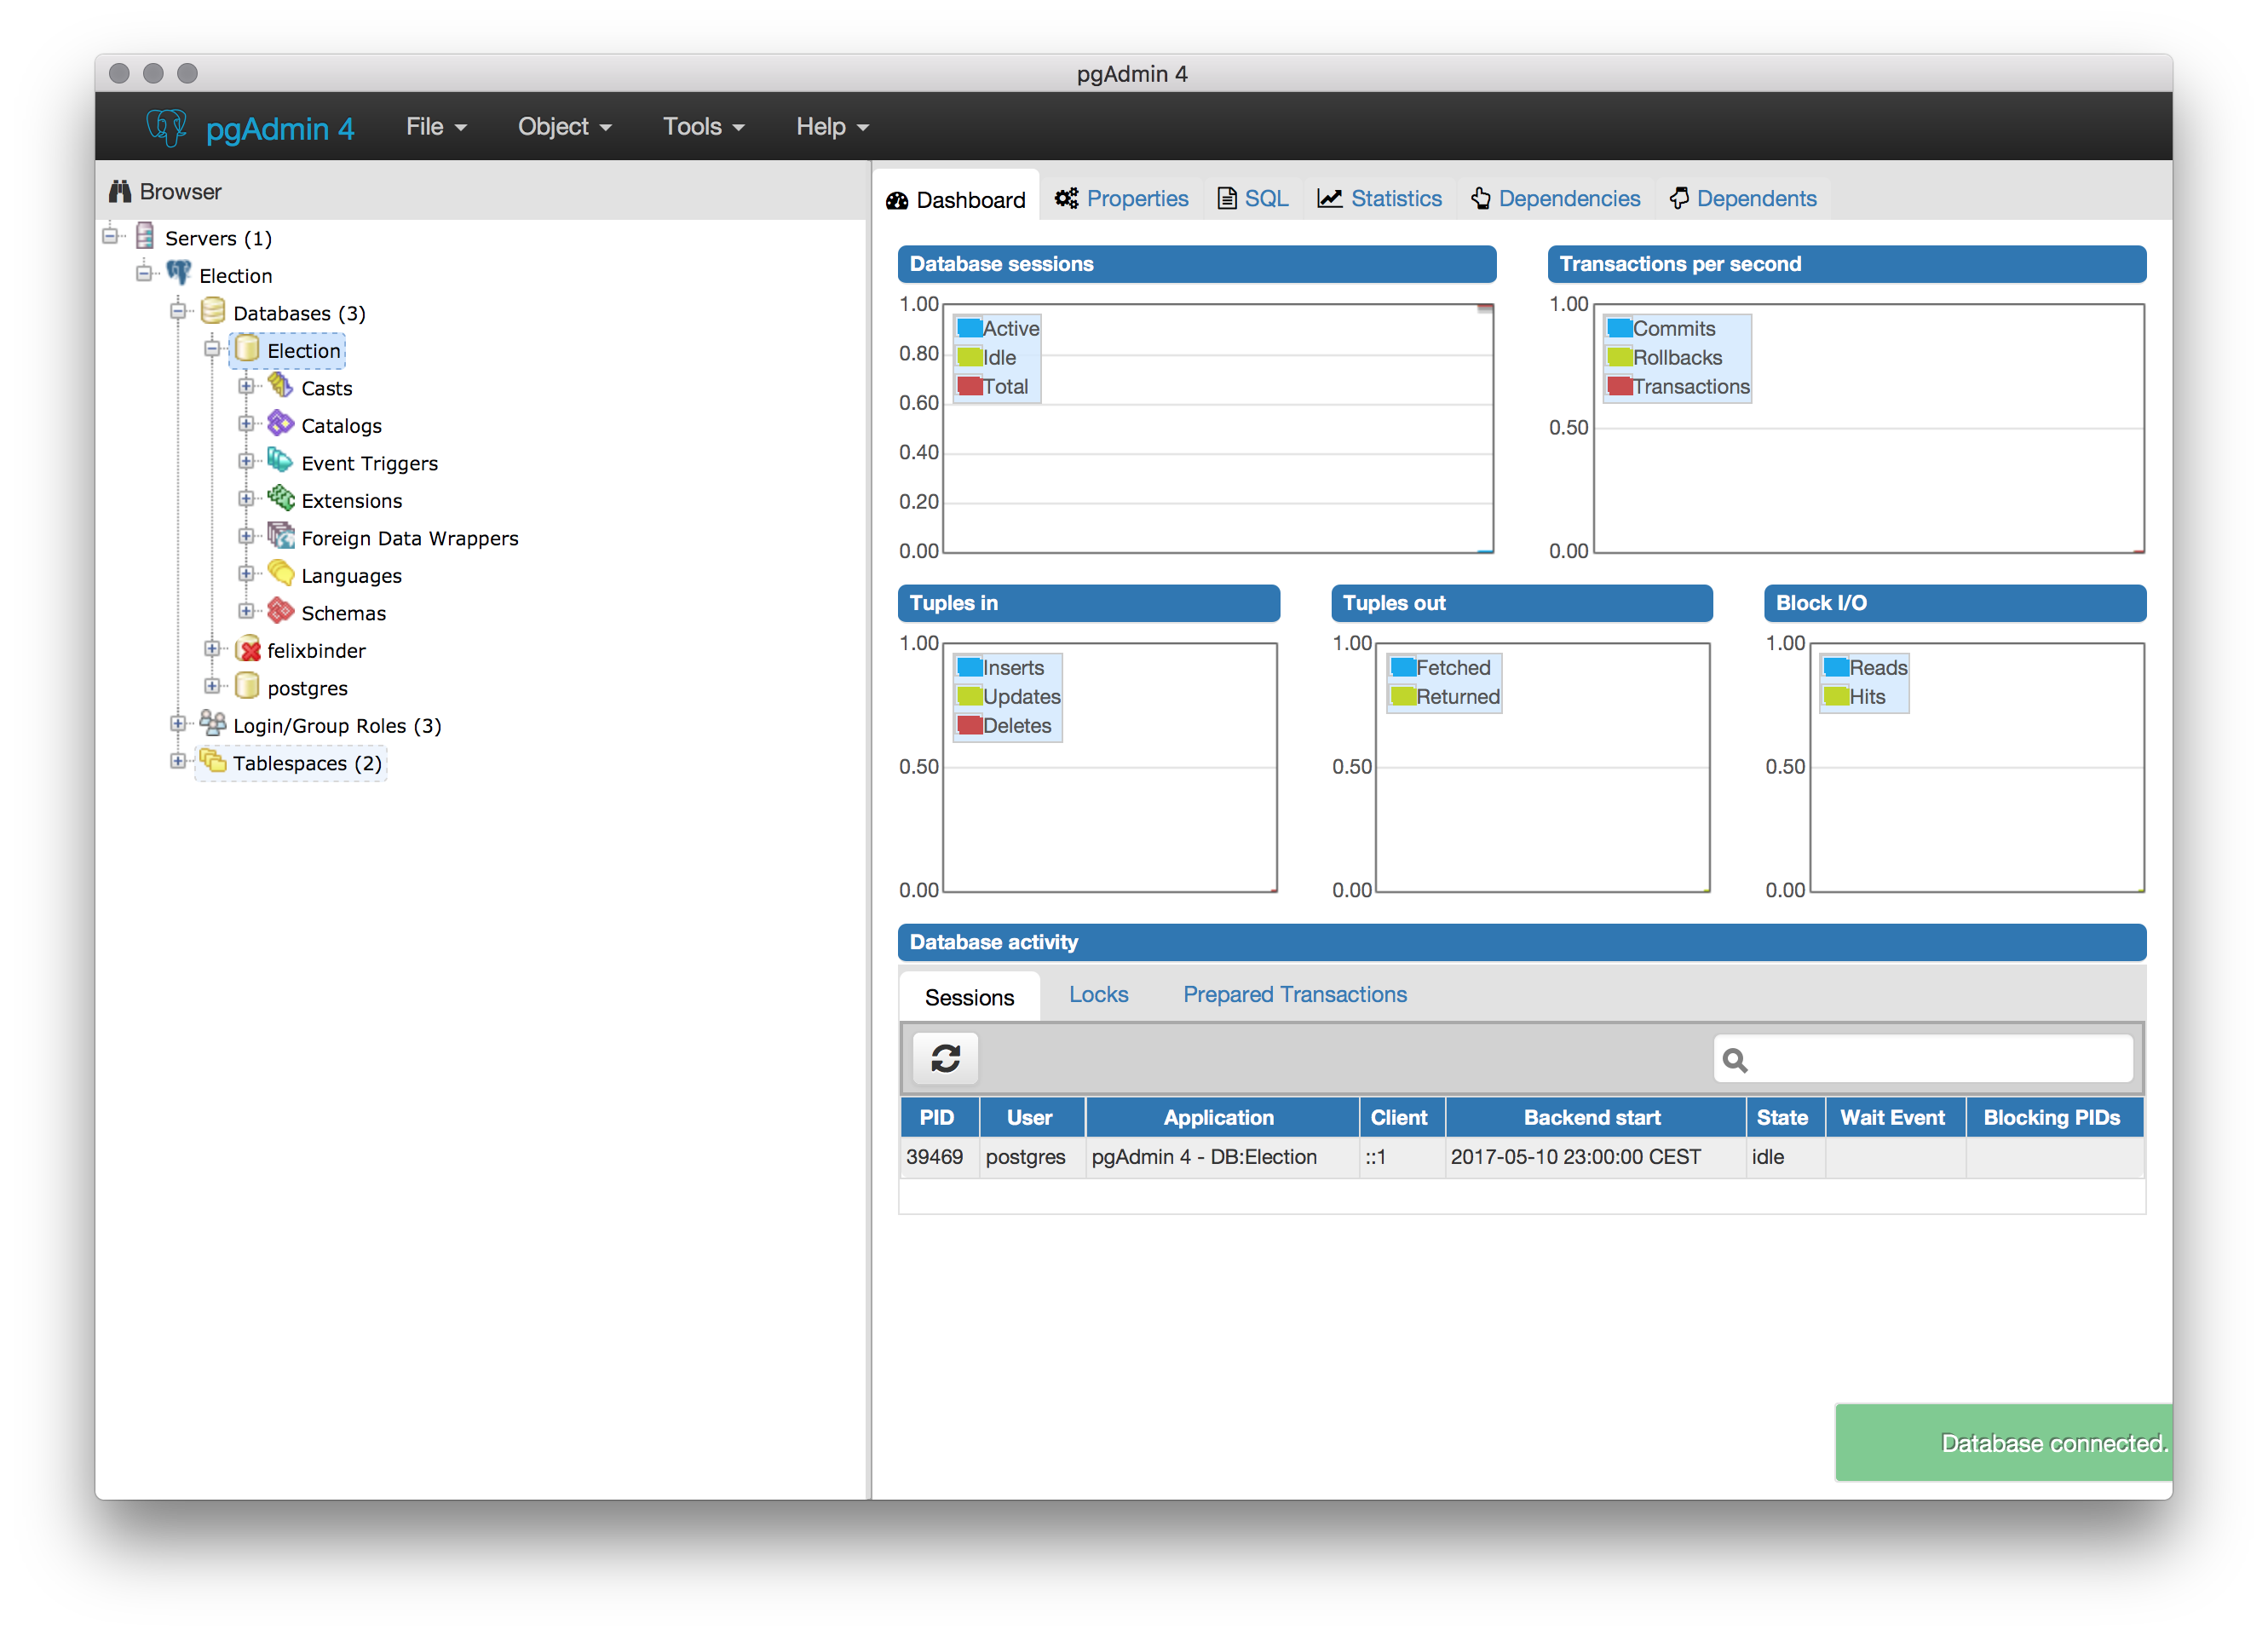
\includegraphics[width=0.95\textwidth]{datenbank_beweis.png}

Der Code dafür war:
\begin{verbatim}
	CREATE DATABASE "Election"
	    WITH 
	    OWNER = postgres
	    ENCODING = 'UTF8'
	    CONNECTION LIMIT = -1;
\end{verbatim}

\subsection{Datenbankschema erstellen}
\url{https://github.com/felixbinder/FU_DBS_Projekt/blob/master/election.sql}

\subsection{Datenbereinigung}
\url{https://github.com/felixbinder/FU_DBS_Projekt/blob/master/Convert.java}

\subsection{Datenimport}
\url{https://github.com/felixbinder/FU_DBS_Projekt/blob/master/Insert.java}

\subsection{Webserver}
Wir haben einen Apache2-Server unter Ubuntu aufgesetzt. Dazu nutzten wir \begin{sffamily}sudo apt-get install apache2\end{sffamily}. Der Server wird mit \begin{sffamily}sudo service apache2 start\end{sffamily} gestartet. Die Konfiguration haben wir unseren Bedürfnissen angepasst.

\subsection{Metrik für Ähnlichkeit von Hashtags}
Wir wählen eine Metrik für die Ähnlichkeit, die auf zeitlicher Ähnlichkeit im Auftreten der Tweets beruht. Der Gedanke dahinter ist, dass zeitlich aufeinanderfolgende Tweets tendentiell thematisch zusammenhängen. Die Metrik sucht für jeden Tweet A den nächsten Tweet B und berechnet den zeitlichen Abstand. Die zeitlichen Abstände werden quadriert, es wird \(\frac{1000}{\text{Distanz}}\) gerechnet, zum bisherigen Ähnlichkeitswert summiert und dann der Durchschnitt gebildet. Somit bildet die Metrik die durchschnittliche quadratische zeitliche Distanz zu einem Auftreten des Hashtags. Die Metrik wird in beide Richtungen berechnet, um die Symmetrieeigenschaft zu wahren.
\begin{python}
[...]
    for htA in hashtags:
        for htB in hashtags:
            print("Berechne: "+str(htA[0])+" und "+str(htB[0]))
        #Berechne Abstand htA und htB 
            final_ae = aehnlichtkeit(htA,htB) + aehnlichtkeit(htA,htB)
            cursor.execute("INSERT INTO hashtags_aehnlichkeit(name1,name2,aehnlichkeit) VALUES('"+str(htA[0])+"','"+str(htB[0])+"',"+str(final_ae)+");")
   [...]
def aehnlichtkeit(htA, htB):
    aehnlichkeit = 0
    count = 0
    cursor.execute("SELECT time FROM tweet, t_enth_h WHERE tweet.ID = t_enth_h.tweet_id AND h_name = '" + str(htA[0]) + "';")
    atweets = cursor.fetchall() #[alle Tweets, die Hashtag A enthalten]
    cursor.execute("SELECT time FROM tweet, t_enth_h WHERE tweet.ID = t_enth_h.tweet_id AND h_name = '" + str(htB[0]) + "';")
    btweets = cursor.fetchall() #[alle Tweets, die Hashtag B enthalten]
    for at in atweets:
        k=0
        distance = []
        for bt in btweets:
            distance.append(float(abs((at[0] - bt[0]).total_seconds())))
        md = min(distance)
        if md == 0:
            aehnlichkeit+100 #Wert waehlen!
        else: 
            aehnlichkeit += 1000/min(distance)
    return aehnlichkeit
\end{python}
Quelldatei: \url{https://github.com/felixbinder/FU_DBS_Projekt/blob/master/metrik_zeit.py}

\subsection{K-Means}
Jeder Hashtags hat nach der Berechnung der Ähnlichkeitsmetrik einen Ähnlichkeitswert zu allen anderen l Hashtags. Jeder Hashtag hat somit einen l-dimensionalen Vektor. Auf Basis dieses Vektors (die zusammen einen Vektorraum aufspannen), der die Ähnlichkeit zu allen anderen Hashtags beschreibt, führen wir k-means aus.

Die Ergebnisse von K-Means werden bei Aufgabe 2.3 visualisiert. Dafür fügt das Skript zur Berechnung von K-Means für jeden Hashtag in die Datenbank zwei Werte ein: erstens den zugehörigen Cluster und zweitens markieren wir die k Hashtags, die für ihren Cluster am repräsentativsten sind. Die berechnen wir, in dem wir für jeden Centroid den Hashtag berechnen, dessen Position im oben beschriebenen Vektorraum am nächsten (euklidische Distanz) zu dem Centroid ist. Dieser repräsentiert dann den Cluster als dessen typischster Vertreter. Der Code findet sich hier: \url{https://github.com/felixbinder/FU_DBS_Projekt/blob/master/Clusterfindung.py}

\subsection{Visualisierung des Hashtagnetzwerks}

\subsubsection{Aufbereitung des Graphens}

Nachdem die Daten aus der Datenbank exportiert wurden und manuell in Excel gereinigt wurden, wird zuerst mithilfe von Gephi ein Graph erstellt in dem alle Hashtags einen Knoten bilden und jedes Hashtag Paar einen Kanten bekommt. Die Graph-Datei befindet sich hier: \url{https://github.com/felixbinder/FU_DBS_Projekt/blob/master/graph.gexf}. Die Visualisierung sieht folgendermaßen aus: \\
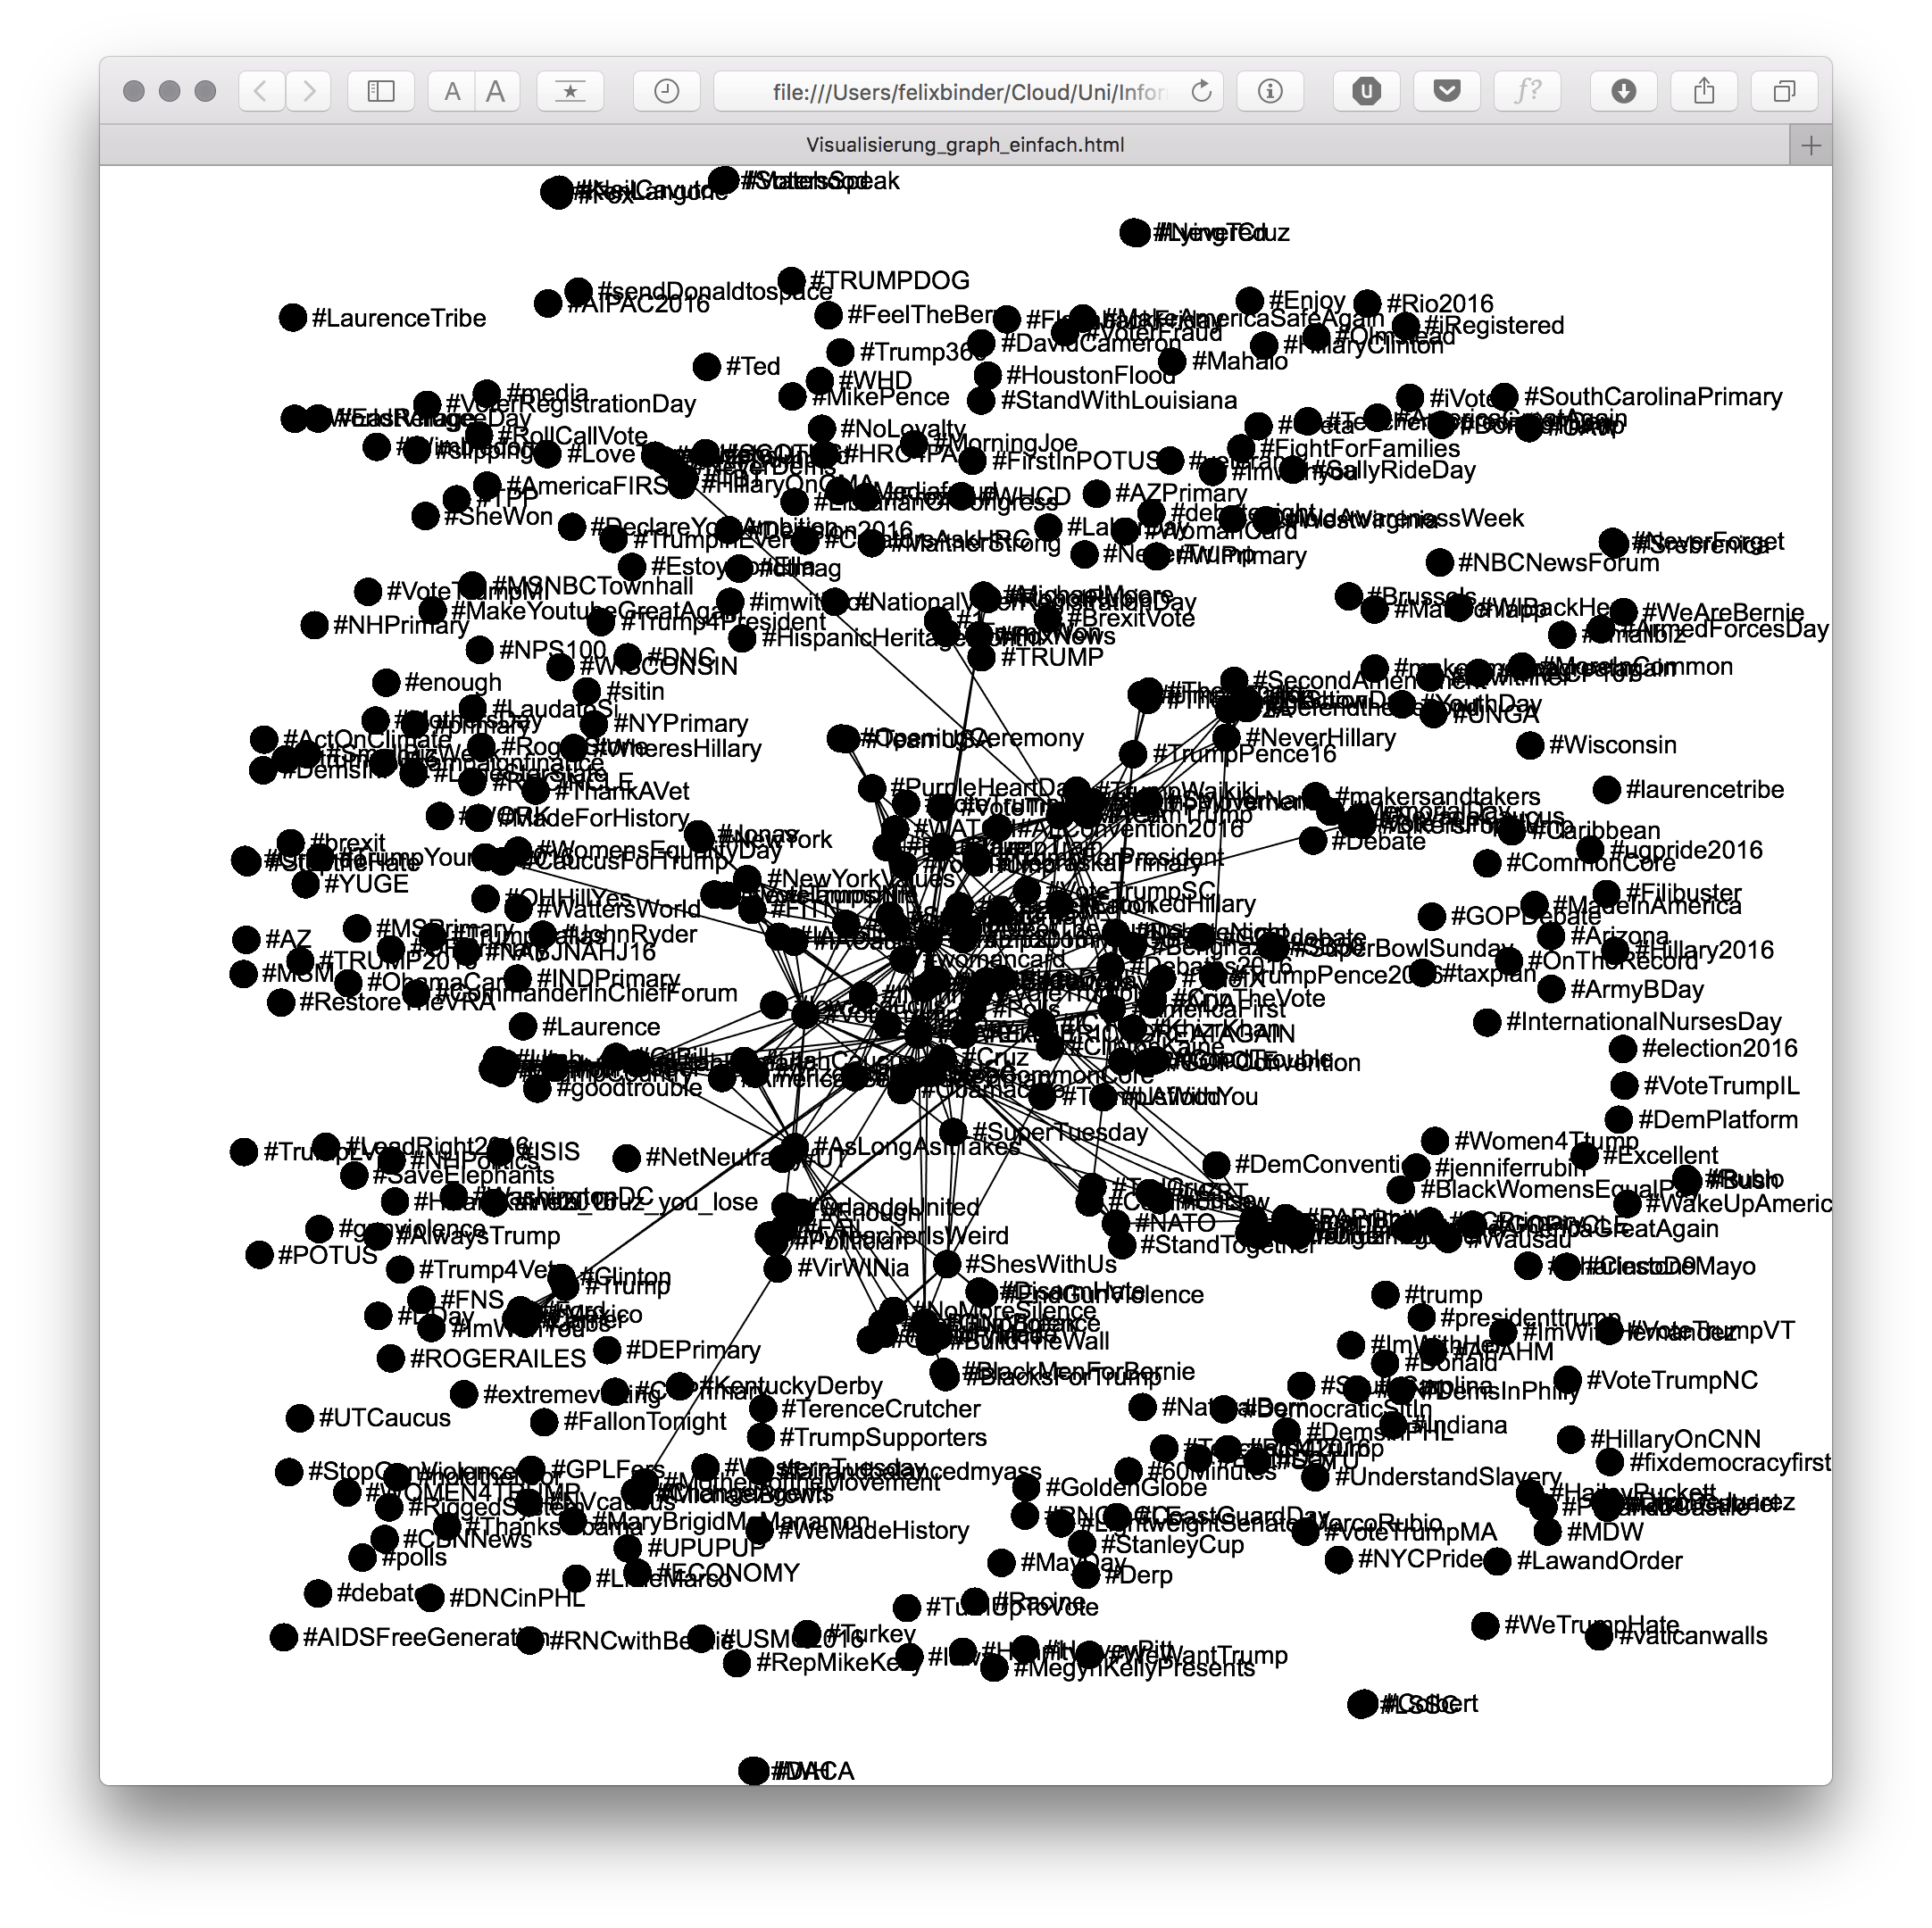
\includegraphics[width=1\textwidth]{2-2visualisierung.png}


Anschließend wurden die Daten entsprechend dem nächsten Schritt (Aufgabe 2-3) zur Visualisierung der Ähnlichkeit aufbereitet. Die Exceltabelle findet sich hier: \url{https://github.com/felixbinder/FU_DBS_Projekt/blob/master/Graph-Rohdaten.xlsx}, die Graph-Datei hier: \url{https://github.com/felixbinder/FU_DBS_Projekt/blob/master/graph_final.gexf}\subsubsection{Visualisierung}
Die Daten werden mit sigma.js visualisiert. Dabei entspricht die Größe des Knoten der absoluten Zahl des Auftretens des entsprechenden Hashtags. Die Farbe der Hashtags entspricht deren Zugehörigkeit zu einem k-means-Clusters. Der repräsentativste Hashtag eines Cluster wird mit einem Diamanten markiert. Der Graph wird mit dem AtlasForce2 Algorithmus visualisert. Dieser Algorithmus ist ein physik-basierter Layout-Algorithmus. Er verwendet die Knoten zwischen Kanten als Federn, deren Gewicht (hier: Ähnlichkeit) deren Stärke beschreibt. Beim Betrachten der Visualisierung kann beobachtet werden, wie die Knoten sich in dem Graphen sich in den ersten Sekunden verschieben, bis schließlich ein Gleichgewicht eingestellt hat und der Graph so gerückt wurde, dass die Knoten nach ihrer Ähnlichkeit (via Kantengewicht) geordnet wurden (wobei nicht zwangsläufigerweise eine optimale Lösung erreicht wird). Die Visualisierung liegt in der Datei \texttt{FU\_DBS\_Projekt/sigma.js/graph viz.html}.\\
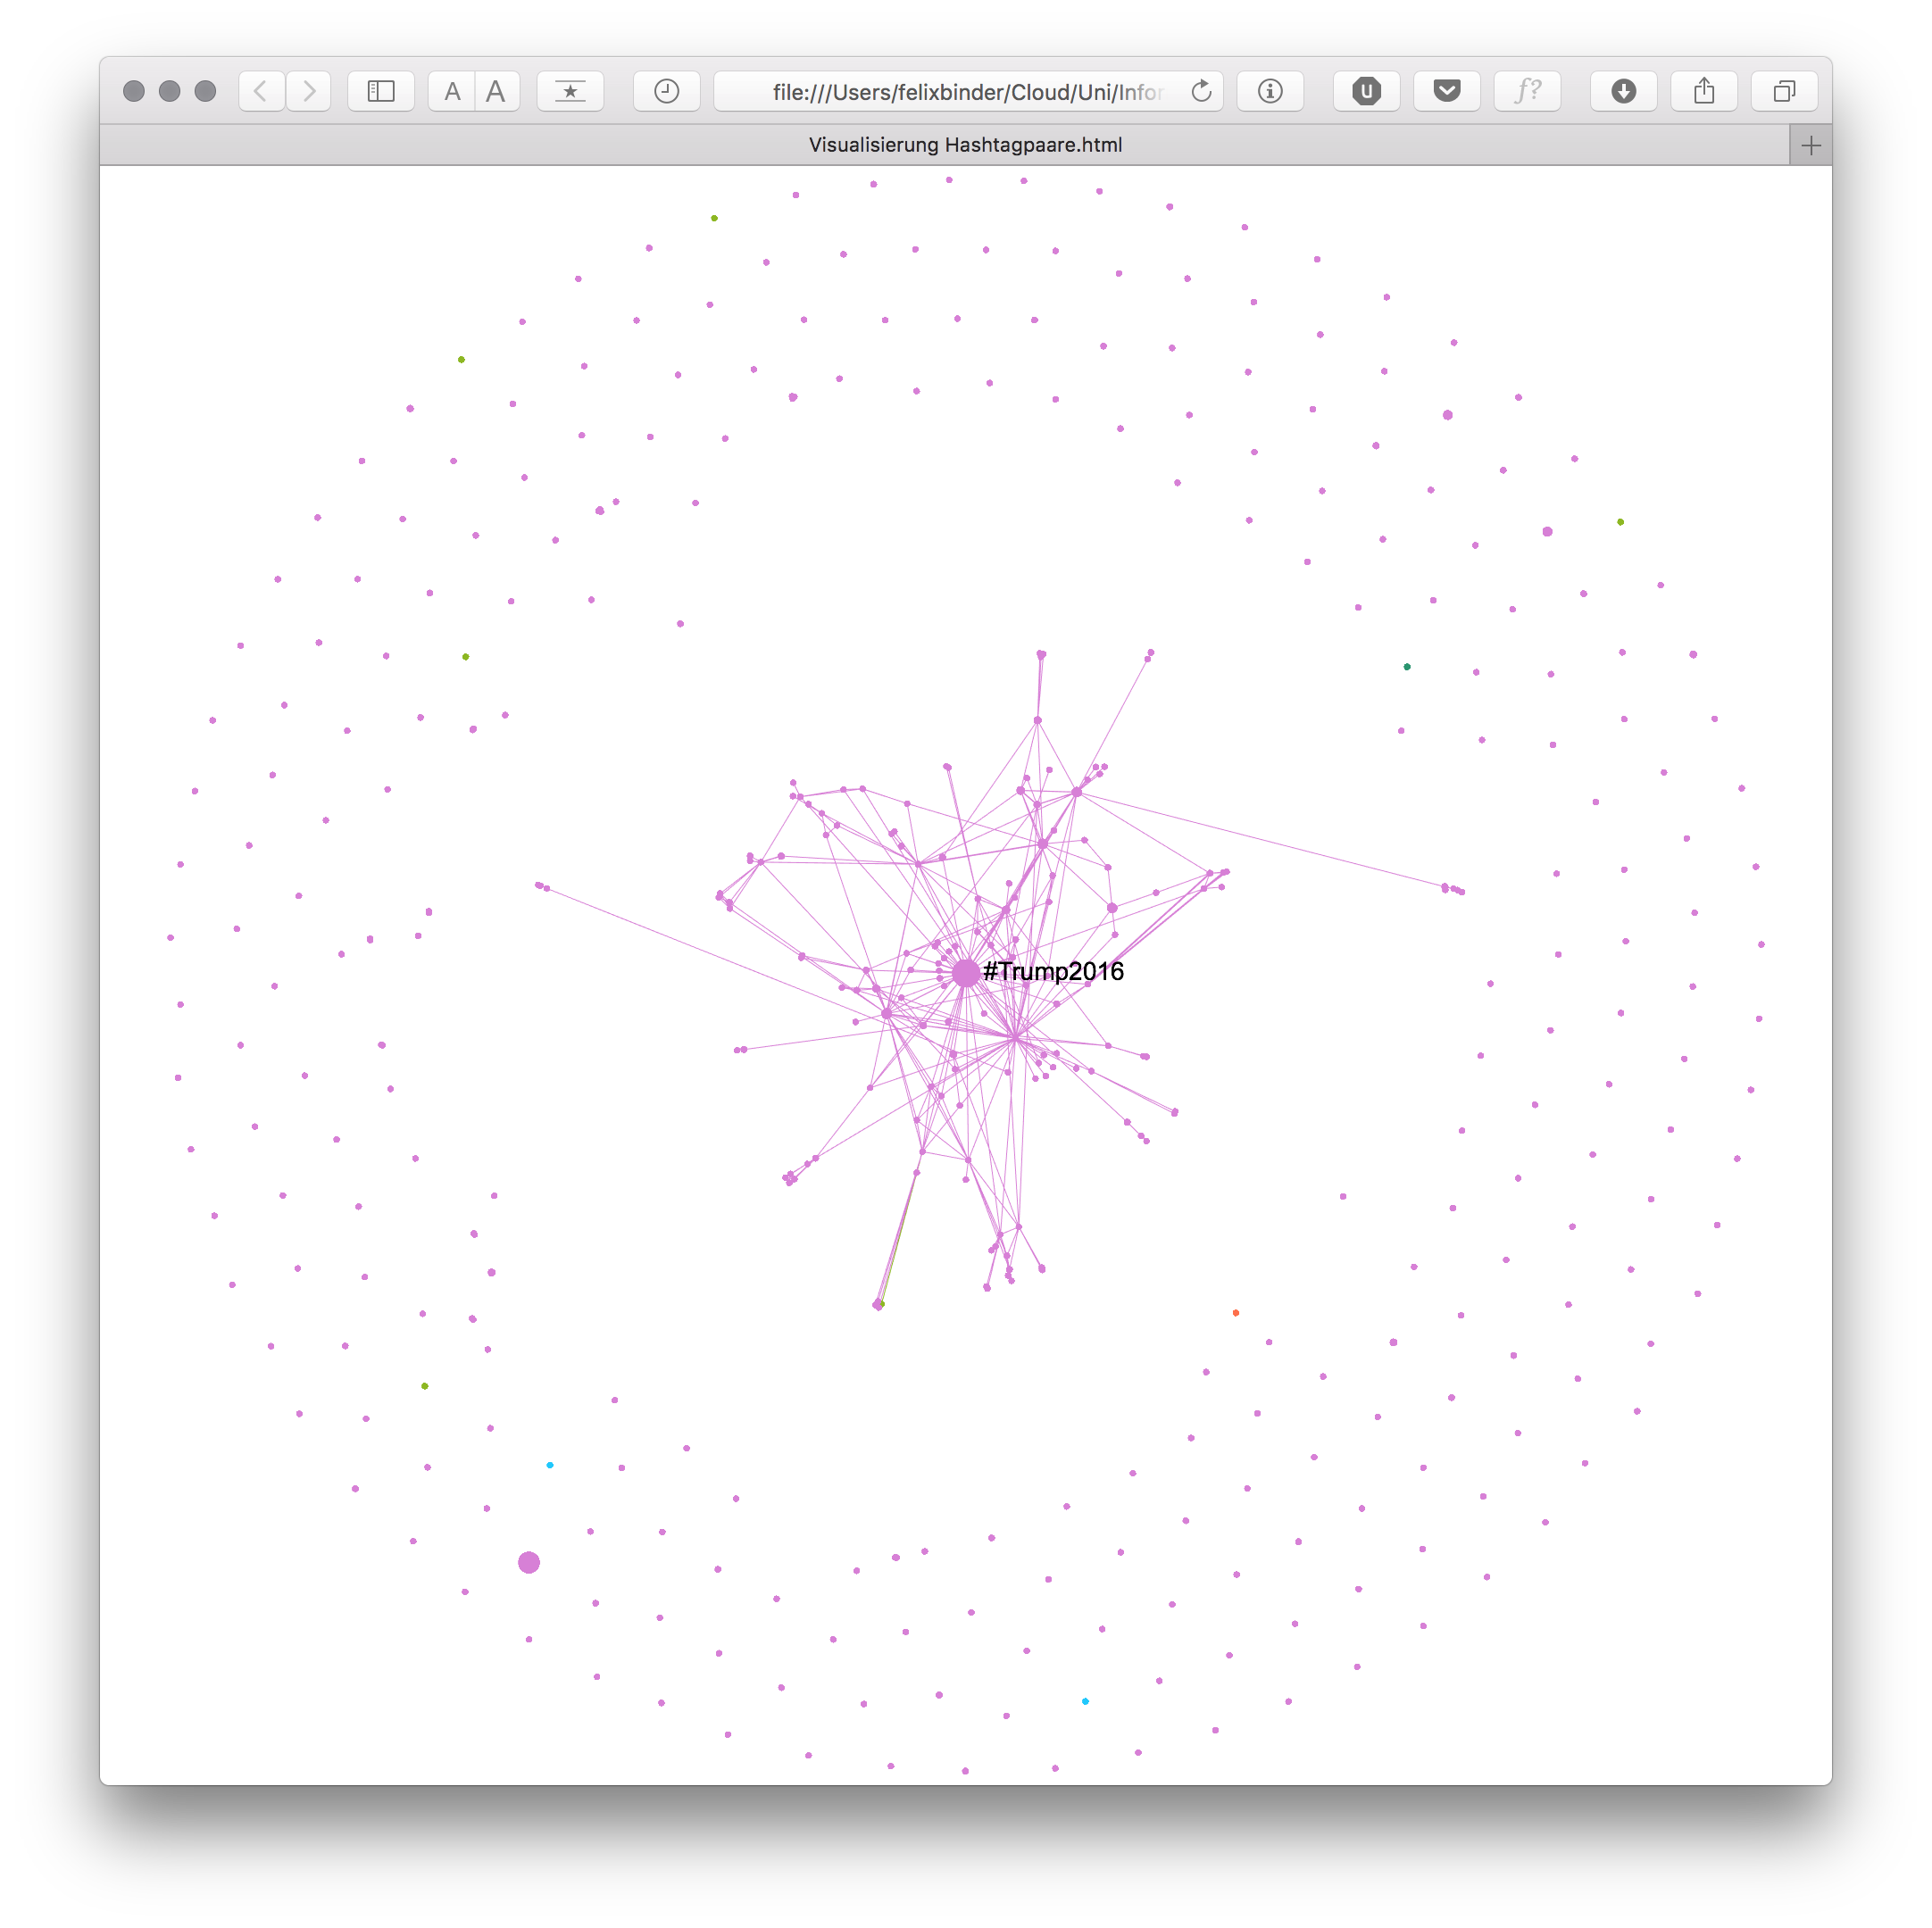
\includegraphics[width=1\textwidth]{visualized.png} Da die Datei auf Bibliotheken von sigma.js zugreift, muss die Ordnerstruktur gewahrt bleiben. Hier die entsprechende Orderstruktur als .zip: \url{https://github.com/felixbinder/FU_DBS_Projekt/blob/master/sigmajs.zip} (es ist zu beachten, dass die Graph"=Datei im selben Verzeichnis wie der Ordner liegen muss).


\subsection{Visualisierung aller Hashtags}

Die Häufigkeit des Autretens aller Hashtags insgesamt über die Zeit hinweg haben wir mittels PHP und JavaScript visualisiert. Der Quellcode ist hier zu finden: \url{https://github.com/felixbinder/FU_DBS_Projekt/blob/master/a2_4.php} Eine Fassung, die alle JavaScript"=Bibliotheken (und auch bereits Aufgabe 2-5) enthält, kann hier heruntergeladen werden: \url{https://github.com/felixbinder/FU_DBS_Projekt/blob/master/Aufgabe_2-4_2-5.tar.gz} Die\linebreak Visualisierung selbst sieht wie folgt aus:

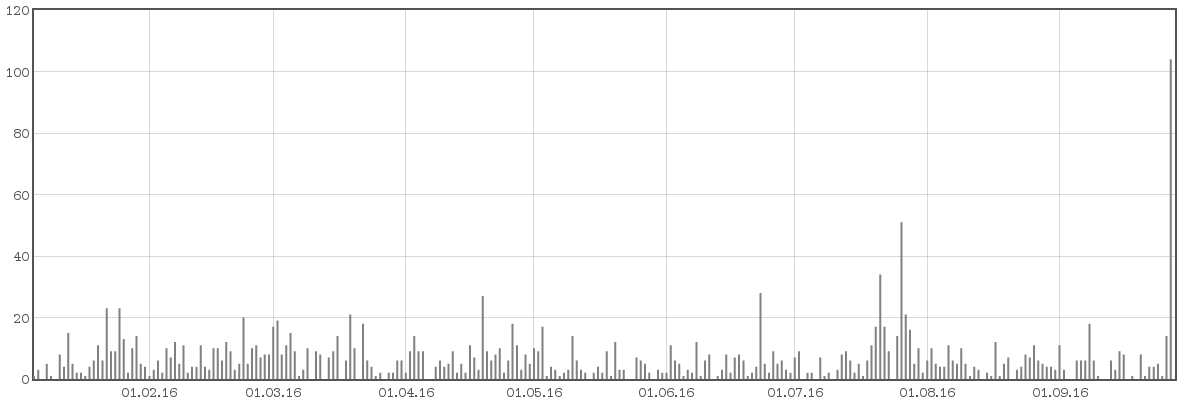
\includegraphics[width=0.95\textwidth]{a2_4.png}

\subsection{Visualisierung einzelner Hashtags}

Die Häufigkeit des Autretens einzelner Hashtags über die Zeit hinweg haben wir mittels PHP und JavaScript visualisiert. Der Quellcode ist hier zu finden: \url{https://github.com/felixbinder/FU_DBS_Projekt/blob/master/a2_5.php} Die Visualisierung selbst sieht wie folgt aus (zwei zufällig ausgewählte Beispiele):

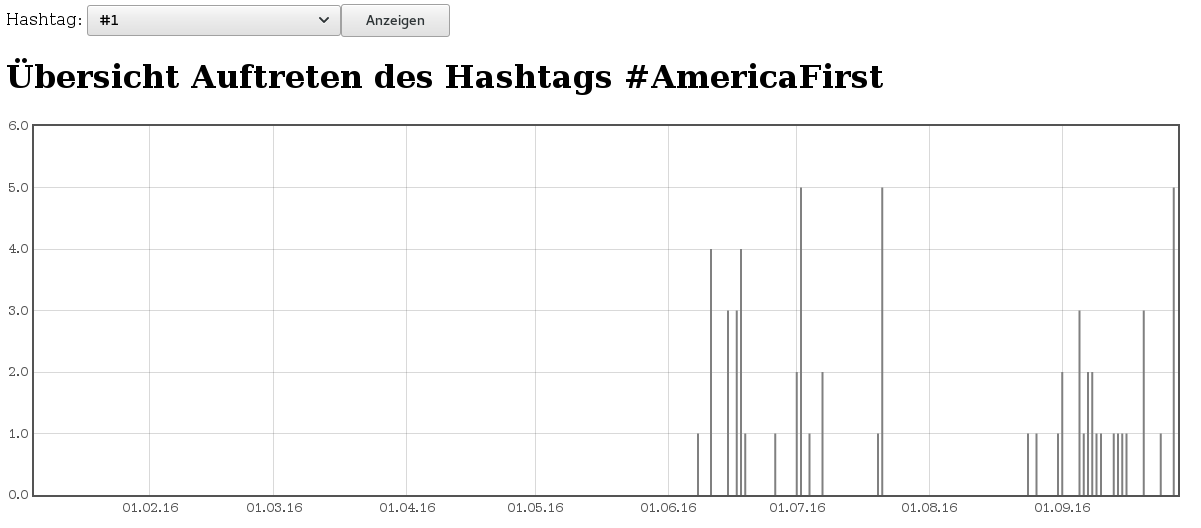
\includegraphics[width=0.95\textwidth]{a2_5_1.png}

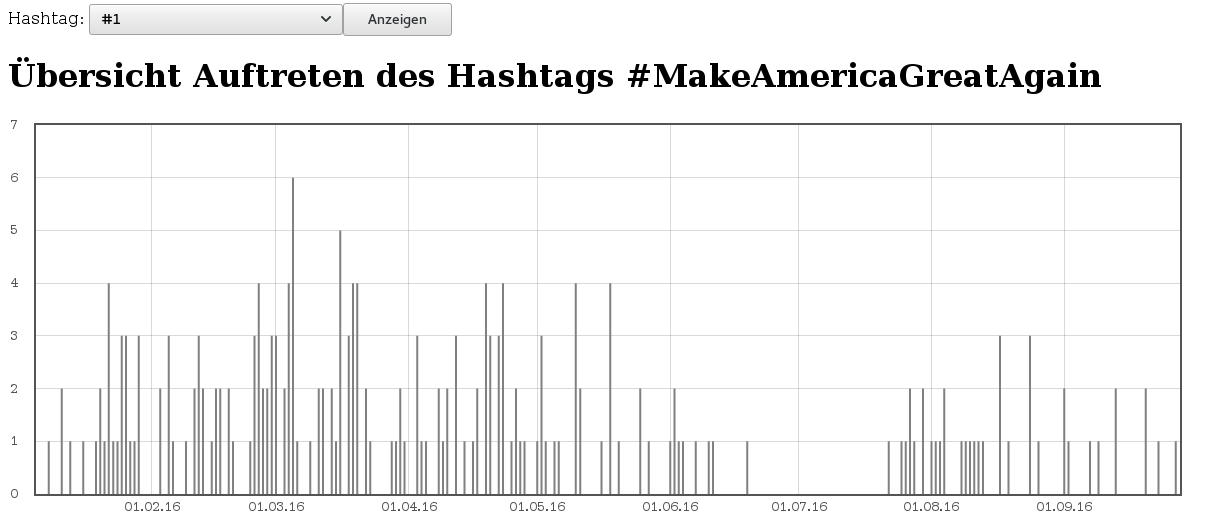
\includegraphics[width=0.95\textwidth]{a2_5_2.png}

\end{document}


